\documentclass[12pt,a4paper]{article}

% Paquetes básicos
\usepackage[utf8]{inputenc}
\usepackage[T1]{fontenc}
\usepackage[spanish]{babel}
\usepackage{amsmath, amssymb}
\usepackage{siunitx} % Ángulos
\usepackage{graphicx}
\usepackage{float}
\usepackage{geometry}
\usepackage{xcolor}
\geometry{margin=2.5cm}
\usepackage{hyperref}
\usepackage{caption}
\usepackage{subcaption}
\usepackage{setspace}
\usepackage{multirow}
\usepackage{minted}  % Códigos
\usepackage{gensymb} % Grados: "°"
\usepackage[backend=biber, style=ieee]{biblatex}
\usepackage{csquotes}
\usepackage{booktabs}
\addbibresource{Bibliografía.bib}
\graphicspath{{Figuras/}}
\onehalfspacing
\hypersetup{
    colorlinks  = true,
    linkcolor   = blue,    
    citecolor   = blue,
    urlcolor    = blue,
    filecolor   = blue
}


\begin{document}       
\renewcommand{\figureautorefname}{Fig.}
\renewcommand{\tableautorefname}{Tab.}
\renewcommand{\equationautorefname}{Ec.}


% Carátula personalizada
\begin{titlepage}
    \centering
    
\includegraphics[width=0.7\textwidth]{Marvell Logo.png}\\[1.5cm]

    {\Large \textbf{PROGRAMA DE FORMACIÓN MARVELL} \\[0.5cm]}
    {\Large Comunicaciones Ópticas} \\[0.5cm]

    \rule{\textwidth}{0.5pt} \\[0.5cm]
    {\Large \textbf{Trabajo Práctico N°2: Fenómenos de las Comunicaciones Ópticas y Ecualización MIMO} \\[0.3cm]}
    \rule{\textwidth}{0.5pt} \\[1cm]
    
\begin{tabular}{l l}
    \textbf{Profesores:} & Francisco Rainero.\\
                         & Nestor Campos.\\
    \\[0.5cm]
    \textbf{Alumnos:} & Monja, Ernesto Joaquín (43.873.728)\\
                      & Zúñiga, Guillermo Rubén Darío (44.229.491)\\
\end{tabular} \\[5cm]

{\centering Año 2026 \par}

\end{titlepage}



% Índice
\tableofcontents
\newpage
%\indent

\section{Introducción}                                              \label{sec_1}
A lo largo de este informe se expande el simulador desarrollado previamente en el Trabajo Práctico N°1, mediante la incorporación de la dispersión cromática (\textit{CD}) del canal óptico. Para mitigar este ensanchamiento temporal, se implementa un \textit{Bulk Chromatic Dispersion Equalizer} (\textit{BCDE}) y se evalúa su exigencia computacional tanto en el dominio del tiempo como en el de la frecuencia.

Posteriormente, la arquitectura del receptor se perfecciona al introducir un ecualizador de espaciado fraccional (\textit{FSE}) para señales \textit{QAM-16}, cuyo entrenamiento intercala un algoritmo de módulo constante (\textit{CMA}) y un esquema dirigido por decisión (\textit{DD}). Por último, el sistema se escala a un esquema \textit{MIMO} $2 \times 2$ para cuantificar su robustez al rastrear y compensar dinámicamente las rotaciones del estado de polarización (\textit{SOP}) presentes en enlaces de doble polarización.



\section{Desarrollo}                                                \label{sec_2}
\subsection{Modelo de \textit{Dispersión Cromática} (CD) y \textit{Bulk Chromatic Dispersion Equalizer} (BCDE)}                   \label{sec_2.1}

La \emph{dispersión cromática} (CD) es un fenómeno de la fibra óptica donde las distintas frecuencias de la señal transmitida viajan a distintas velocidades, generando un desfasaje mayor a las componentes de más altas frecuencias. La respuesta en frecuencia de la \textit{CD} esta dada por la \autoref{eq_1},
\begin{equation}
    H_{CD} (\Omega) = {e^{j \frac{\beta_2}{2} L_f \Omega^2}}
    \label{eq_1}
\end{equation}

\noindent
donde $\beta_{2}$ es el parámetro de dispersión y $L_{f}$ es la longitud de la fibra. El problema de este efecto es que tiene un retardo de grupo lineal, sin embargo y como esta respuesta tiene módulo 1, es posible compensar esta distorsión utilizando un ecualizador con criterio de \emph{Zero Forcing}. Este ecualizador se denomina \emph{Bull Chromatic Dispersion Equalizer} (BCDE).

Se realizó un script en \textit{Python} \cite{b1} que grafica la fase de esta respuesta en frecuencia según distintas longitudes de fibra junto con la respuesta del \textit{BCDE}. Este gráfico se muestra en la \autoref{fig:fig_1}. A partir de esto se puede concluir lo siguiente:
\begin{itemize}
    \item Si $L_{f} = 0$ entonces no se modela la fibra, por lo que la respuesta es plana.
    \item La respuesta de fase depende linealmente de la longitud para una frecuencia fija.
    \item La respuesta forma una parábola, por lo que ésta depende de la frecuencia de la señal al cuadrado.
\end{itemize}

\begin{figure}[H]
    \centering
    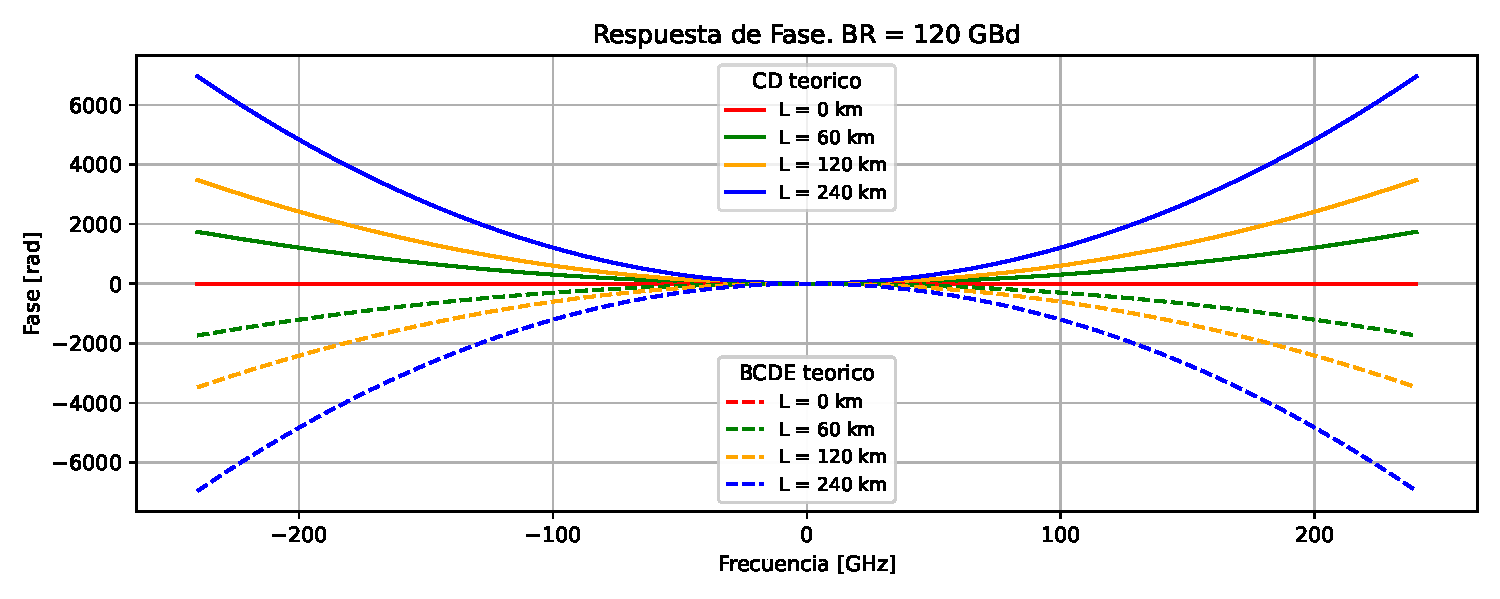
\includegraphics[width=\linewidth]{Figura 1.pdf}
    \caption{Fase de la respuesta en frecuencia del \textit{CD} y el \textit{BCDE} según $L_{f}$.}
    \label{fig:fig_1}
\end{figure}

Con el script se graficó además la respuesta según el \textit{Baudrate} ($BR$) de la transmisión en la \autoref{fig:fig_2}. En ella se observa que un mayor $BR$ provoca una mayor penalización por dispersión, ya que el espectro abarca más curvatura de fase. Por lo tanto, al subir el \textit{Baudrate}, se requiere más compensación en el canal, por el crecimiento de la diferencia de fase entre componentes espectrales.

\begin{figure}[b!]
    \centering
    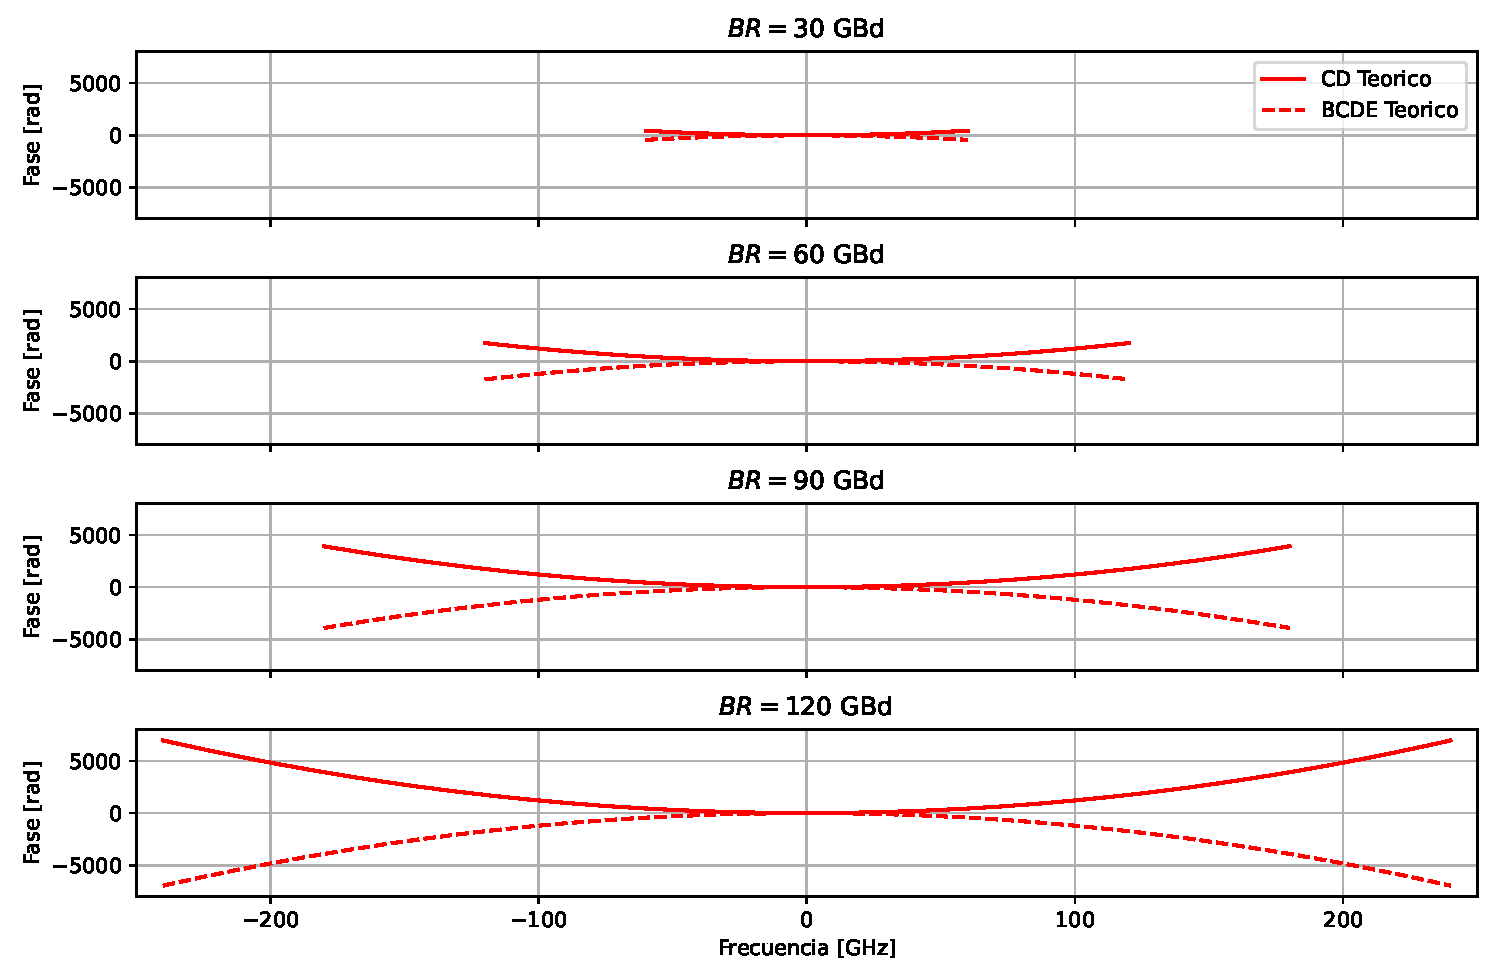
\includegraphics[width=0.9\linewidth]{Figura 2.pdf}
    \caption{Respuesta del \textit{CD} y el \textit{BCDE} según $BR$. $L_f=240$\,km}
    \label{fig:fig_2}
\end{figure}

Un detalle que se puede apreciar en los gráficos es que el \textit{BCDE} cancela de forma exacta al \textit{CD}, logrando eliminar el efecto en el receptor. Se espera entonces que el efecto de la fibra no afecte el Bit Error Rate (\textit{BER}) en un sistema de comunicaciones.

Se graficó mediante \textit{Python} la \autoref{fig:fig_3}, que compara la \textit{BER} con distintas longitudes de fibra, la \textit{BER} teórica y la \textit{BER} sin fibra. Se observa efectivamente que la curva no cambia a excepción de un $E_{b}/N_{0}$ bajo, y esto es porque en la simulación se generaron directamente los símbolos y cada error de símbolo se contó como error de 1 bit, por lo que se esperó tener una \textit{BER} menor a la teórica. Se concluye entonces que el fenómeno es totalmente reversible, sin importar la longitud de la fibra.

\begin{figure}[t]
    \centering
    
\includegraphics[width=0.8\linewidth]{Figura 3.pdf}
    \caption{Curvas de BER con modelo de fibra.}
    \label{fig:fig_3}
\end{figure}

Por otro lado, el numero de taps del \textit{BCDE} necesario para lograr la reversión, depende de la dispersión máxima, que a su vez depende de la longitud de la fibra y el Baudrate. Es decir:
\begin{equation}
    N_{TAPS} = \frac{f_s\cdot CD_{max}\cdot BR\cdot \lambda_0^2}{c}
    \label{eq_2}
\end{equation}

\noindent
donde $\lambda_{0}$ es la longitud de onda, $c$ es la velocidad de la luz y $CD_{max}$ es la dispersión cromática máxima, que se define según la \autoref{eq_3}, como:
\begin{equation}
    CD_{max} = D\cdot L_{max}
    \label{eq_3}
\end{equation}

\noindent
donde $L_{max}$ es la longitud total de la fibra.

Utilizando \textit{Python} se calculó número de taps según la longitud de fibra y el Baudrate, con los resultados mostrados en la \autoref{fig:fig_4}. El número de taps necesarios del \textit{BCDE} crece linealmente con la longitud de la fibra y con el Baudrate. Para una misma distancia, un Baudrate más alto exige más taps porque la señal ocupa una banda más ancha y se requiere compensar más dispersión.

También se observa que, a bajas longitudes, el número de taps es bajo y el filtro es implementable, pero al combinar longitudes grandes con Baudrates elevados, la complejidad es mayor y el filtro no puede ser implementado. En particular, para $90$ y $120 \ [GBd]$ el número de taps aumenta rápidamente hasta valores muy altos, lo que implica una carga de hardware excesiva.

\begin{figure}[t]
    \centering
    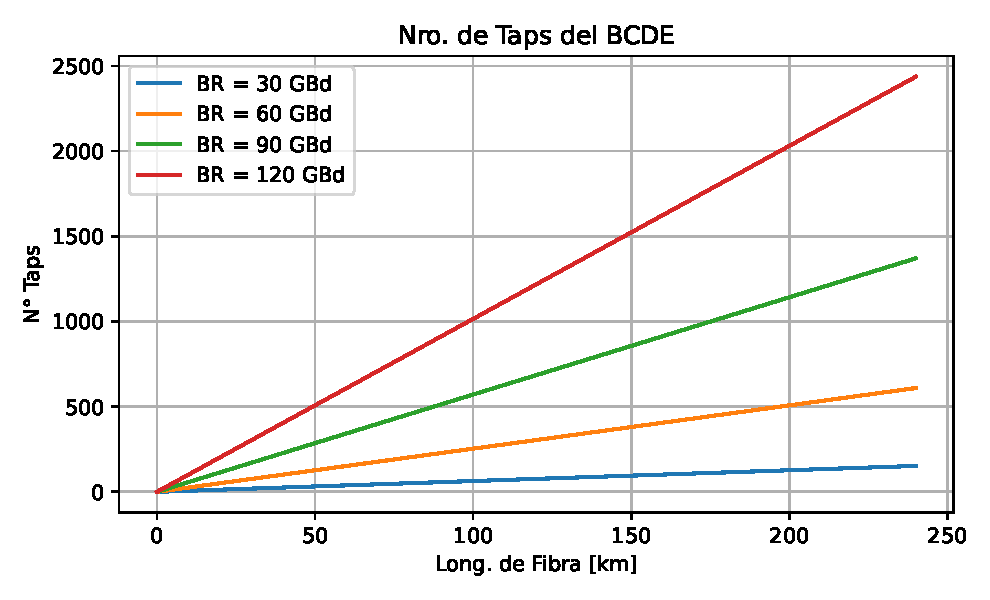
\includegraphics[width=0.75\linewidth]{Figura 4.pdf}
    \caption{Cantidad de taps del BCDE según $L_f$ y $BR$.}
    \label{fig:fig_4}
\end{figure}

El \textit{BCDE} puede implementarse en el dominio del tiempo o de la frecuencia, donde la cantidad de multiplicaciones requeridas en el tiempo esta dada por la \autoref{eq_4}:
\begin{equation}
    C_{TD} = 4 \, N_{TAPS}^{2}
    \label{eq_4}
\end{equation}

\noindent
mientras que en frecuencia, la cantidad de multiplicaciones estará dada según la \autoref{eq_5}:

\begin{equation}
    C_{FD} = 4\,N_{TAPS}\,(3\log_2(N_{TAPS}) + 5) + 1000
    \label{eq_5}
\end{equation}

Estas ecuaciones se graficaron en la \autoref{fig:fig_5}. Se puede apreciar que la implementación en el tiempo es más conveniente hasta los $30$ taps, luego, para más de $30$ taps es recomendable la implementación en frecuencia.

Se realizó un acercamiento a la \autoref{fig:fig_6} para determinar a partir de qué valores de $L_{f}$ y $BR$ se utiliza la implementación \textit{FD}. Estos valores se encuentran en el \autoref{tab:tab_1}.
\begin{table}[H]
    \centering
    \begin{tabular}{@{} ccc @{}}
        \toprule
        \textbf{Baudrate [GBd]} & \textbf{Long. de Fibra [km]} \\
        \midrule
         30 & $45.7$ \\
         60 & $11.4$ \\
         90 & $5$    \\
        120 & $2.8$  \\
        \bottomrule
    \end{tabular}
    \caption{Longitud de fibra máxima para implementar el \textit{BCDE} en el tiempo, según $BR$.}
    \label{tab:tab_1}
\end{table}

\begin{figure}[H]
    \centering
    \begin{minipage}{0.49\linewidth}
        \centering
        
\includegraphics[width=\linewidth]{Figura 5.pdf}
        \caption{Cantidad de multiplicaciones según el número de taps del \textit{BCDE}.}
        \label{fig:fig_5}
    \end{minipage}
    \hfill
    \begin{minipage}{0.49\linewidth}
        \centering
        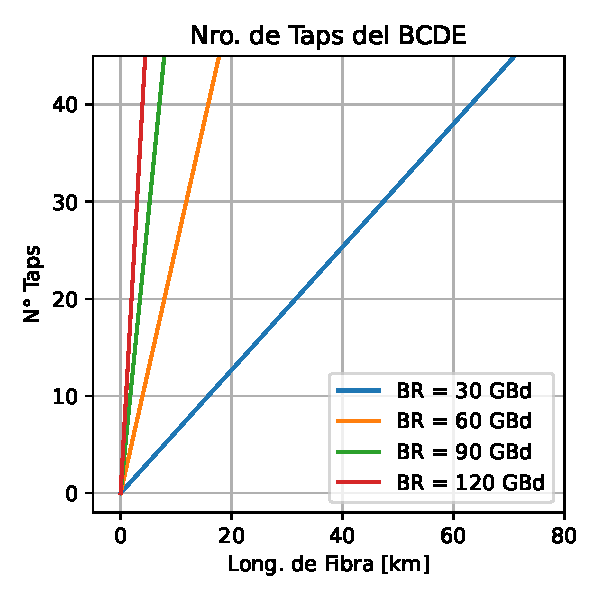
\includegraphics[width=\linewidth]{Figura 6.pdf}
        \caption{Acercamiento de la \autoref{fig:fig_4} a $N_{taps} = 30$.}
        \label{fig:fig_6}
    \end{minipage}
\end{figure}



\subsection{Análisis de Desempeño del Ecualizador \textit{FSE} en \textit{QAM-16}} \label{sec_2.2}
En esta sección se evalúa el comportamiento de un ecualizador de espaciado fraccional (\textit{FSE}) implementado para mitigar la interferencia intersímbolos (\textit{ISI}) en un sistema de comunicaciones que emplea modulación \textit{QAM-16} basándonos en una adaptación y mejora del Ejercicio 4 del TP1 en \textit{Python} \cite{b2}. El entrenamiento del \textit{FSE} se divide en dos etapas fundamentales: una fase inicial ciega utilizando el algoritmo de módulo constante (\textit{CMA}) para asegurar la apertura del diagrama de ojo, seguida de una fase dirigida por decisión (\textit{DD}) para minimizar el error en estado estacionario.


\subsubsection{Sensibilidad al Paso de Adaptación y Tamaño del Ecualizador} \label{sec_2.2.1}
Para comprender la dinámica de convergencia, se realizó un barrido conjunto del paso de adaptación ($\mu$) durante la fase \textit{DD} y del número de coeficientes del ecualizador ($N_{taps}$). La \autoref{fig:fig_7} ilustra la penalidad de $SNR$ en dB (medida a un $BER = 10^{-3}$) en función de $\log_{2}(\mu)$.

A partir de las curvas obtenidas, se puede afirmar que \textbf{sí existe un valor óptimo de $\mu$ para cada tamaño de ecualizador}, el cual se evidencia en el punto mínimo del ``valle'' de cada curva. A su vez, se observa una fuerte relación entre el tamaño del filtro y su sensibilidad: los ecualizadores de mayor tamaño ($N_{taps} = 127$ y $255$) presentan un rango operativo de $\mu$ sumamente estrecho. Un paso de adaptación muy pequeño impide que el algoritmo converja en el tiempo simulado, mientras que un paso muy grande provoca la divergencia rápida del filtro debido a la amplificación del ruido de gradiente.

\begin{figure}[t]
    \centering
    
\includegraphics[width=1\textwidth]{Figura 7.png} 
    \caption{Penalidad de SNR vs. $\log_2(\mu)$ para distintos tamaños de ecualizador, con y sin limitación de ancho de banda ($BW$).}
    \label{fig:fig_7}
\end{figure}

Al introducir una limitación de ancho de banda ($BW$) previa a la etapa de ruido en el canal, el piso general de la penalidad se eleva y los valles se desplazan ligeramente. Esto evidencia que el ecualizador debe invertir un mayor esfuerzo para compensar la severa distorsión del canal. Ocurre entonces que los tamaños de ecualizador intermedios, particularmente el de $N_{taps} = 63$, demuestran ser los más robustos. Ofrecen un excelente equilibrio entre la capacidad para invertir el canal y un margen de estabilidad amplio para el paso de adaptación, superando el desempeño inestable del filtro de $N_{taps} = 255$.


\subsubsection{Impacto Visual: Análisis de Constelaciones}          \label{sec_2.2.2}
Para ilustrar el trabajo interno del algoritmo, se seleccionó un caso robusto determinado en el punto anterior ($N_{taps} = 63$, $\mu = 2^{-7}$) operando bajo la condición limitante de ancho de banda. 
\begin{figure}[H]
    \centering
    
\includegraphics[width=0.8\textwidth]{Figura 8.png}
    \caption{Constelaciones de la señal recibida antes y después de la ecualización FSE en un entorno con ancho de banda limitado.}
    \label{fig:fig_8}
\end{figure}

Como se aprecia en la parte izquierda de la \autoref{fig:fig_8}, la señal que ingresa al receptor presenta una severa dispersión, fusionando las fronteras de decisión de los símbolos de la constelación \textit{QAM-16} y dificultando la correcta decodificación por parte del \textit{slicer}. Tras el paso por el \textit{FSE} (véase la parte derecha de la \autoref{fig:fig_8}), la constelación recupera su estructura clásica, agrupando la energía nítidamente en torno a los 16 puntos ideales de la modulación y demostrando la efectividad de la compensación.


\subsubsection{Dinámica de Convergencia: Curva de Aprendizaje}      \label{sec_2.2.3}
Finalmente, la transición temporal y analítica entre los algoritmos de entrenamiento se observa mediante la curva de aprendizaje del filtro, presentada en la \autoref{fig:fig_9}.
\begin{figure}[H]
    \centering
    
\includegraphics[width=0.9\textwidth]{Figura 9.png}
    \caption{Curva de aprendizaje del ecualizador mostrando la evolución del error cuadrático medio y la transición de la fase \textit{CMA} a \textit{DD}.}
    \label{fig:fig_9}
\end{figure}

Durante las primeras iteraciones (a la izquierda de la marca de conmutación), el algoritmo \textit{CMA} logra estabilizar los pesos y reducir el error de manera sostenida basándose únicamente en la estadística de módulo constante, sin requerir una secuencia de entrenamiento. 

En el punto exacto de conmutación, el algoritmo transiciona al modo Dirigido por Decisión (\textit{DD}). Se observa entonces una caída abrupta y profunda del Error Cuadrático Medio. Este salto valida que el ecualizador habría alcanzado el régimen suficiente durante la etapa ciega (\textit{CMA}) para que las decisiones del \textit{slicer} fuesen en su gran mayoría correctas, permitiendo al modo \textit{DD} realizar el ajuste preciso final y llevar el filtro a su estado estacionario óptimo.



\subsection{Ecualizador FSE \emph{MIMO} y Rotación del \emph{Estado de Polarización} (SOP)}                                            \label{sec_2.3}
A modo de extensión del simulador con FSE desarrollado en la sección \ref{sec_2.2}, se incorporó un soporte a un esquema \emph{MIMO} (Multiple Input, Multiple Output) que utilizan los DSP cuando se transmiten señales utilizando las dos polarizaciones ortogonales de la luz (polarización H y V). La utilización de esta propiedad de la luz implica también tener en cuenta el fenómeno de la \emph{rotación del estado de polarización} (SOP), que mezcla las dos componentes de polarización. La velocidad a la que el SOP rota se denomina \emph{frecuencia de rotación} ($f_{SOP}$).

Para este caso, se utilizó un simulador con un FSE MIMO $2\times 2$ brindado en el curso y realizado en Matlab, con la diferencia de que fue traducido a Python para mantener la coherencia con los demás scripts desarrollados anteriormente \cite{b3}. Este simulador incorpora un modelo de canal de fibra que contiene el modelo de SOP junto con los demás fenómenos vistos en el cursado, tales como la CD, la DGD (differential group delay) y la PMD (polarization mode dispersion); pero que en este caso no se trabajaron para poder diferenciar los efectos que la rotación del SOP produce junto a diferentes pasos de ecualización del FSE $2\times 2$.

Utilizando este simulador, se realizó un barrido de la $f_{SOP}$ y el paso del ecualizador $\mu$ para calcular la \emph{penalidad de SNR} con $BER = 10^{-3}$. Para este caso se utilizó el mismo $\mu$ en el algoritmo CMA y DD.

El resultado de este barrido se muestra en la figura \ref{fig:fig_10}, donde se observa que el paso con menor penalidad es de $0.002$ para hasta $30$\,kHz de rotación, luego pasa a ser $0.004$ y finalmente $0.006$ para altas frecuencias. Por otro lado, la penalidad se degrada significativamente a partir de $60$\,kHz pero solo para $\mu = 0.002$.

\begin{figure}[H]
    \centering
    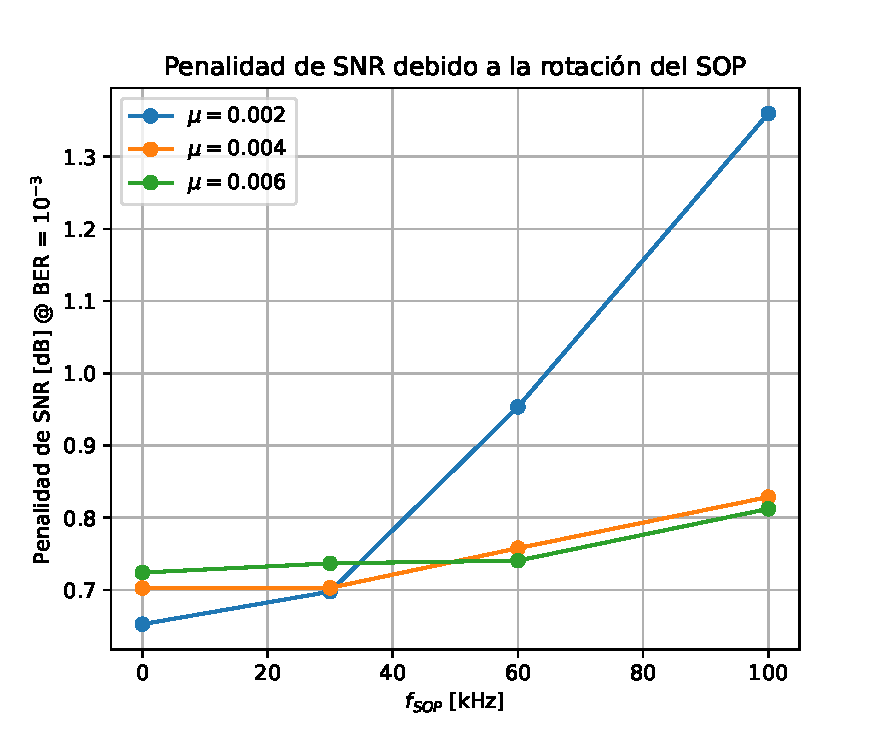
\includegraphics[width=0.6\textwidth]{Figura 10.pdf}
    \caption{Curva de penalidad de SNR según $f_{SOP}$ y $\mu$.}
    \label{fig:fig_10}
\end{figure}

A partir de estas observaciones, se pueden extraer las siguientes conclusiones:

\begin{itemize}
    \item No existe un $\mu$ óptimo que minimice la penalidad para todo el rango de $f_{SOP}$, sino que el óptimo cambia según $f_{SOP}$.
    \item La penalidad comienza a degradarse a baja frecuencia solo si $\mu$ es muy bajo; se estima que a más alta frecuencia (200\,kHz) la penalidad aumenta más para $\mu$ más grande.
    \item La capacidad de seguimiento (\emph{tracking}) del algoritmo DD se ve empeorada mientras sube la $f_{SOP}$, porque si $\mu$ es muy bajo, las muestras pueden caer en el slicer sobre una región de decisión distinta a la que deberían y los símbolos se desfasan $90^\circ$ en la constelación. El algoritmo no ve este cambio de alineación ya que solo optimiza el filtro para que la salida tenga la forma de un QAM-16.
\end{itemize}

\section{Conclusiones}                                              \label{sec_3}
Se estudiaron los ecualizadores BCDE, FSE unidimensional y FSE escalado a MIMO. El BCDE compensa de forma exacta el efecto de la CD, sin impacto en el BER, pero con una complejidad de implementación que crece linealmente con la longitud de fibra y el baudrate. Por otro lado, se observó cómo el algoritmo CMA del FSE abre el diagrama de ojo para luego refinar la convergencia con el algoritmo DD; también se observó que existe un valor óptimo de $\mu$ para cada tamaño de filtro. Cuando el FSE se extiende a un sistema MIMO, el $\mu$ óptimo depende de la $f_{SOP}$ y la capacidad de seguimiento del algoritmo DD corre riesgo de degradarse a altas frecuencias debido a desalineaciones de 90° en la constelación.

\newpage
\printbibliography[heading=bibintoc, title={4. \ Referencias}]

\end{document}